% Please make sure you insert your
% data according to the instructions in PoSauthmanual.pdf
\documentclass[a4paper,11pt]{article}
\usepackage{pos}

\usepackage{xfrac}
\usepackage{siunitx}
\usepackage[size=tiny]{todonotes}
\presetkeys{todonotes}{color=blue!30}{}


\ShortTitle{Physics updates of the simulation tool PROPOSAL}
\title{Physics updates of the high-energy lepton and photon simulation tool PROPOSAL}

\author*[a]{Jean-Marco Alameddine}
\author[a]{Pascal Gutjahr}
\author[a]{Wolfgang Rhode}
\author[b]{Alexander Sandrock}
\author[a]{Jan Soedingrekso}

\affiliation[a]{Technische Universität Dortmund, Fakultät Physik,\\
  Otto-Hahn-Straße 4a, 44227 Dortmund, Germany}

\affiliation[b]{Bergische Universität Wuppertal,
  Fakultät für Mathematik und Naturwissenschaften,\\
  Gaußstraße 20, 42119 Wuppertal, Germany}


% Uncomment \onbehalf{...} for collaboration if you want.
%\onbehalf{for the XXXX collaboration} 

% In this case, you also have to uncomment the lines after "%Full authors list" below and include the full authors list,

\emailAdd{jean-marco.alameddine@tu-dortmund.de}
\emailAdd{pascal.gutjahr@tu-dortmund.de}
\emailAdd{wolfgang.rhode@tu-dortmund.de}
\emailAdd{asandrock@icecube.wisc.edu}
\emailAdd{jan.soedingrekso@tu-dortmund.de}

\abstract{
Monte Carlo simulations are an important tool in modern physics experiments. With improving detector sensitivities, higher accuracies are also required from simulations, for example in reconstruction tasks. This includes both correctness from a physical as well as an algorithmic point of view. PROPOSAL is a Monte Carlo simulation framework that provides three-dimensional simulations of high-energy photons, electrons, muons, and taus. It is written in C++, but can also be used within Python via a wrapper. The structure of the software allows for simple customization of the propagation environment, physics descriptions, or precision settings for a variety of use cases. Examples are the application in neutrino observatories, underground experiments, or air shower simulations. This contribution focuses on the recent physics updates of the framework, describing the methodology and implication of these improvements. In particular, this involves effects at the higher and lower end of the energy scale covered by PROPOSAL. For high-energy photons, photon-nucleon interactions, muon pairproduction, and the Landau-Pomeranchuk-Migdal effect in electron-positron pairproduction are now included. As lower-energy effects, the deflection of muons in stochastic interactions as well as an approximate description of the photoeffect for photons have been implemented.}

\ConferenceLogo{PoS_ICRC2023_logo.pdf}

\FullConference{%
38th International Cosmic Ray Conference (ICRC2023)\\
  26 July - 3 August, 2023\\
  Nagoya, Japan}



%% \tableofcontents

\begin{document}
\maketitle


\section{Introduction}

Modern experiments in physics rely on methods of statistical data analysis to interpret their measurements.
To train these methods, a statistically sufficient dataset where the true properties are known is required.
Especially in astroparticle physics, this can only be achieved using simulations which model the reality.
One of these simulation tools is the framework PROPOSAL \cite{KOEHNE20132070}, which provides a three-dimensional Monte Carlo simulation of high-energy particles propagating through large volumes\footnote{PROPOSAL is available as an open-source C\texttt{++}/Python software under \url{https://github.com/tudo-astroparticlephysics/PROPOSAL}. It can be installed with \texttt{pip install proposal} or via CMake.}.
Originally, PROPOSAL has been written for the simulation of muon and tau leptons in the context of underground observatories, such as the IceCube Neutrino Observatory \cite{IceCube:2021uhz}, or for radio neutrino detectors \cite{PhysRevD.102.083011}.
To be able to use PROPOSAL for the simulation of electromagnetic cascades, a recent update introduced pair production and Compton scattering as photon interactions, annihilation as a new positron interaction, and new dedicated parametrizations to describe ionization and bremsstrahlung losses of electrons and positrons \cite{Alameddine:2021iq}.
With these updates, PROPOSAL could be used to simulate the electromagnetic component of extensive air showers, as it is done in the air shower simulation framework CORSIKA~8 \cite{icrc2023}. 

In this contribution, the implementation of additional photon interaction processes is presented.
This includes photoelectric absorption, photonuclear interactions, muon pair production, and a description of the Landau-Pomeranchuk-Migdal suppression in electron-positron pair production.
These processes are important to describe photons as low energies ($E \lessapprox \SI{0.1}{\mega\electronvolt}$ in air) and very-high energies ($E \gtrapprox \SI{1e18}{\electronvolt}$ in air), as well as due to their distinct event signatures.
\section{Physics improvements for photon interactions}

\begin{figure}
	\centering
    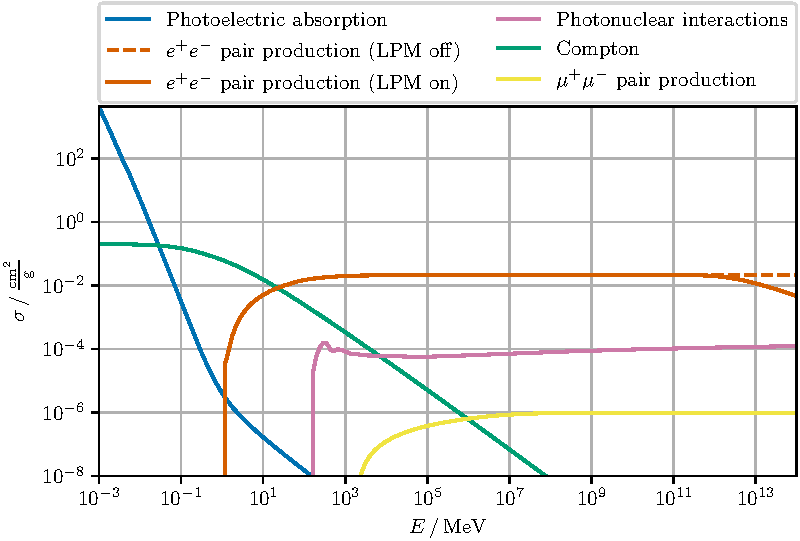
\includegraphics{plots/Photon_Air_dndx_ecut_0.pdf}
    \caption{Total cross section of photons in air inside PROPOSAL.}
    \label{fig:total_cross_photon}
\end{figure}


\subsection{Photoelectric absorption}

Photoelectric absorption describes the ejection of an atomic electron due to its interaction with an in-going photon.
In this process, the photon energy is used to free the electron from its atomic binding, while the remaining photon energy serves as the kinetic energy of the now free electron.
For photons in air, photoelectric absorption becomes the dominant interaction process for energies below $\approx \SI{30}{\kilo\electronvolt}$.
In the context of electromagnetic cascades, photoelectric absorption as a process starts to become important for energies where its cross section represents a significant correction to the total mean free path length.

The detailed description of photoelectric absorption is non-trivial and dependent on the properties of the atomic structure of the interaction target.
Since other codes to describe these processes already exist, PROPOSAL only provides an approximate description based on the cross section given in \cite{heitler, sauter}.
The total cross section is defined as
%
\begin{align}
	\label{eqn:sauter}
	\sigma &= 4 \pi r_e^2 Z^5 \alpha^4 F_1 F_2 \left( \frac{m_e}{E} \right)^5 \left( \gamma^2 -1 \right)^{\sfrac{3}{2}} \left[ \frac{4}{3} + \frac{\gamma (\gamma - 2)}{\gamma + 1} \left( 1 - \frac{\ln{\left( \gamma + \sqrt{\gamma^2 - 1} \right)}}{\gamma \sqrt{\gamma^2 - 1}}  \right) \right],
\end{align}
%
with the photon energy $E$ and the definitions
\begin{align}
	\gamma &= 1 + \frac{E - I}{m_e}, & I &= \frac{Z^2 \alpha^2 m_e}{2}.
\end{align}
%
The term
\begin{align}
	F_1 &= \left[ 1 + \left( \frac{\alpha Z}{\beta} \right)^2 \right] \frac{\pi \alpha Z / \beta }{\sinh(\pi \alpha Z / \beta )} \exp\left[ \frac{\alpha Z}{\beta} \left( \pi - 4 \arctan\left( \frac{\beta}{\alpha Z} \right) \right) \right]
\end{align}
%
is used as a correction factor for the non-relativistic energy regime \cite{sauter}, while the term
%
\begin{align}
	F_2 &= 1 + 0.01481 \ln^2{Z} - 0.000788 \ln^3{Z}
\end{align}
%
is an empirical correction describing the ratio between the K-shell and total photoelectric absorption cross section \cite{hubbell1969}.

The photoelectric cross section and a validation of the total photon cross section at low energies is shown in Figure \ref{fig:photoeffect_nist}, where the total photon cross section in air is compared to the calculations from the NIST Standard Reference Database.
The agreement is at worst \SI{10}{\percent}.

\begin{figure}
	\centering
    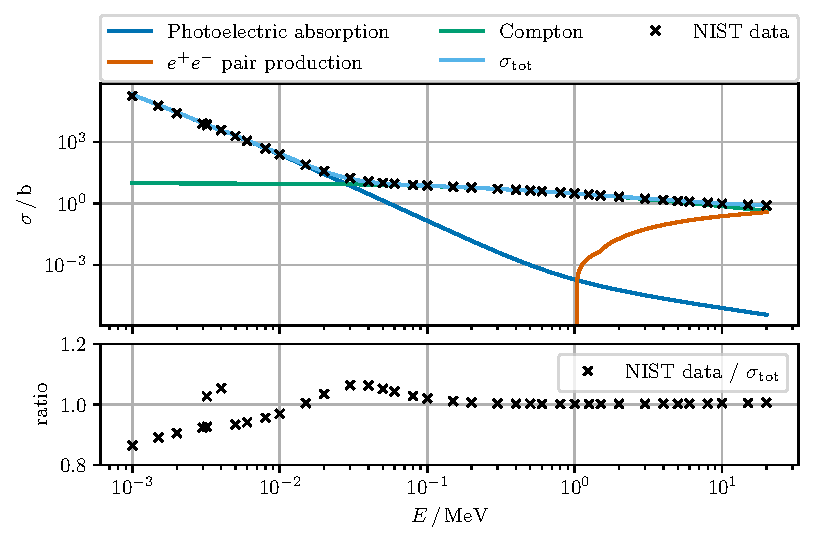
\includegraphics{plots/photoeffect_nist.pdf}
    \caption{Photon cross sections in air for small energies, compared to the total cross section according to the NIST Standard Reference Database.}
    \label{fig:photoeffect_nist}
\end{figure}

\subsection{Photonuclear interactions}


\begin{align}
	\label{eqn:photonuclear_C7}
	\sigma_{\gamma,N} &=
	\begin{cases}
		\left(73.3 s^{0.073} + 191.7 s^{-0.602} \right) \sqrt{1 - s_0 / s} \si{\micro\barn}, & \text{for } \sqrt{s} \leq \SI{19.39}{\giga\electronvolt}, \\
		\left( 59.3 s^{0.093} + 120.2 s^{-0.358} \right) \si{\micro\barn}, & \text{for } \sqrt{s} > \SI{19.39}{\giga\electronvolt}, \\
	\end{cases}
\end{align} 

with the squared center of mass energy $s = m_n^2 + 2 m_n \nu$ and the pion production threshold $\sqrt{s_0} = \SI{1.0761}{\giga\electronvolt}$.

\todo{Shadowing???}

\begin{figure}
	\centering
    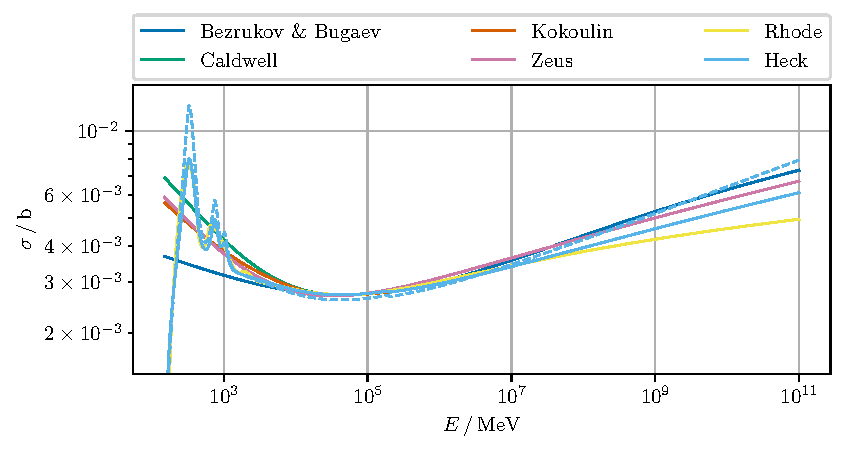
\includegraphics{plots/photoproduction_cross.pdf}
    \caption{Photonuclear interaction cross sections.}
    \label{fig:photoproduction_cross}
\end{figure}


\subsection{Muon pair production}

Muon pair production describes the conversion of a photon to a muon pair in the field of an atomic nucleus.
While its contribution to the mean free path length of photons is negligible compared to the dominant electron positron pair production, the process provides a source of muons from the electromagnetic shower component and therefore a potentially interesting event signature in extensive air showers.

Based on the muon bremsstrahlung cross section given in \cite{Kelner:288828}, the muon pair production cross section is given by
%
\begin{align}
	\begin{split}
		\frac{\mathrm{d}\sigma}{\mathrm{d}x} &= 4 Z^2 \alpha \left( r_e \frac{m_e}{m_\mu} \right)^2 \left[ 1 - \frac{4}{3} (x - x^2) \right] \\ &\times \Biggl( \Phi(\delta) + \frac{1}{Z} \left[ \ln\left( \frac{m_\mu / \delta}{\delta m_\mu / m_e^2 + \sqrt{e}} \right) - \ln\left( 1 + \frac{1}{\delta \sqrt{e} B^\prime Z^{\sfrac{-2}{3}} / m_e} \right) \right] \Biggr),
	\end{split}
\end{align}
%
where
%
\begin{align}
	\Phi(\delta) &= \underbrace{\ln \left( \frac{B Z^{\sfrac{-1}{3}} m_\mu / m_e}{1 + B Z^{\sfrac{-1}{3}} \sqrt{e} \delta / m_e } \right)}_{\Phi_0} - \underbrace{\ln\left( \frac{D_n}{1 + \delta (D_n \sqrt{e} - 2) / m_\mu} \right)}_{\Delta_\text{n}},
\end{align}
%
with the radiation logarithm constant $B$ and the definitions
%
\begin{align}
	x &= \frac{E_{\mu^-}}{E}, & \delta &= \frac{m_\mu^2}{2 E x (1 - x)}, & D_n &= 1.54 A^{0.27}.
\end{align}
%
For $Z > 1$, the effect of the inelastic nuclear form factor is included with the substitution
%
\begin{align}
	\Delta_\text{n} &\rightarrow \left( 1 - \frac{1}{Z} \right) \Delta_\text{n}.
\end{align}
%
The total cross section of muon pair production is shown in Figure \ref{fig:total_cross_photon}.

\subsection{Landau-Pomeranchuk-Migdal effect in electron-positron pair production}

The Landau-Pomeranchuk-Migdal is a suppression of bremsstrahlung and pair production processes occuring when the formation length reaches interatomic distances, which comes in effect for high energies and dense media.
The suppression is effective for small energy losses in case of bremsstrahlung, and for symmetric pair production events in case of electron-positron pair production.

Based on the parametrization of the LPM effect in \cite{RevModPhys.71.1501}, the suppression of the pair production cross section is given by
%
\begin{align}
	\label{eqn:lpm_photopair}
	\frac{\mathrm{d}\sigma_\text{LPM}}{\mathrm{d}x} &= \frac{\mathrm{d}\sigma}{\mathrm{d}x} \cdot \frac{\xi(s) / 3 \left(G(s) + 2 \left( x^2 + (1 - x)^2 \right) \phi(s) \right)}{1 - 4 / 3 x (1 - x)},
\end{align}
%
with $x = E_{e^{-}} / E$, where $E$ is the photon energy.
The functions $\xi(s)$, $G(s)$, $\phi(s)$, are given by \cite{PhysRevD.25.1291, PhysRev.103.1811}
%
\begin{align}
	\xi(s) &\approx \xi(s^\prime) =
	\begin{cases}
		2 & \text{if $s^\prime < s_1$}, \\
		1 + h - \frac{0.08 (1 - h) (1 - (1-h)^2)}{\ln{(s_1)}} & \text{if $s_1 \leq s^\prime < 1$}, \\
		1 & \text{if $s^\prime \geq 1$},
	\end{cases}
\end{align}
%
\begin{align}
	G(s) &=
	\begin{cases}
		3\psi(s) - 2\phi(s) & \text{if $s < \num{0.710390}$}, \\
		36s^2 / \left(36s^2 + 1 \right) & \text{if $\num{0.710390} \leq s < \num{0.904912}$}, \\
		1 - 0.022s^{-4} & \text{if $s \geq \num{0.904912}$},
	\end{cases}
\end{align}
%
\begin{align}
	\psi(s) &= 1 - \exp{\left\{ -4s - \frac{8s^2}{1 + 3.936s + 4.97s^2 - 0.05s^3 + 7.5 s^4} \right\}},
\end{align}
%
\begin{align}
	\phi(s) &=
	\begin{cases}
		1 - \exp{\left\{ -6s \left(1 + (3 - \pi) s\right) + \frac{s^3}{ 0.623 + 0.796s + 0.658 s^2} \right\}} & \text{if $s < \num{1.54954}$}, \\
		1 - 0.012 s^{-4} & \text{if $s \geq \num{1.54954}$},
	\end{cases}
\end{align}
%
with the variable definitions
%
\begin{align}
	s &= \frac{s^\prime}{\sqrt{\xi(s^\prime)}}, & s^\prime &= \frac{1}{8} \sqrt{\frac{E_\text{LPM}}{E x ( 1 - x)}}, & s_1 &= \frac{\sqrt{2} Z^{\sfrac{2}{3}}}{B^2}, \\ E_\text{LPM} &= \frac{2 \alpha (m_e c^2)^2 X_0}{\pi \hbar c}, & h &= \frac{\ln{(s^\prime)}}{\ln{(s_1)}}, & D_n &= 1.54 A^{0.27},
\end{align}
%
where $X_0$ is the radiation length and $B$ the radiation logarithm constant.

Figure \ref{fig:lpm_photopair_diff} shows the effect of the LPM on the differential pair production cross section at different energies.
As expected, for $x = 0.5$, the suppression becomes maximal, while for $x=0$ and $x=1$, the suppression is zero.
Since the LPM effect depends on the material density, its suppression also depends on the height in the Earth's atmosphere.
In Figure \ref{fig:lpm_photopair_cross}, the suppression of the pair production cross section at different atmospheric heights is shown.
%
\begin{figure}
\centering
\begin{minipage}[t]{.48\textwidth}
  \centering
  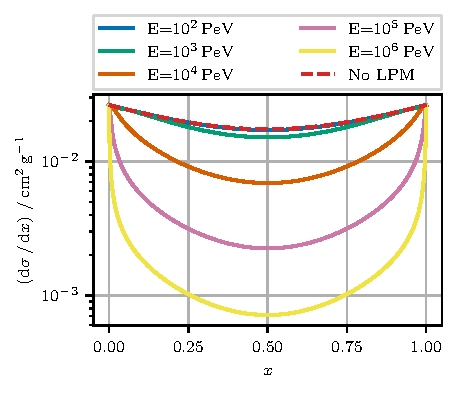
\includegraphics{plots/lpm_photopair_differential_small.pdf}
  \captionof{figure}{Differential cross section for electron-positron pair production in air at standard density, with nitrogen as an interaction target. The effect of the LPM effect at different energies is shown. Note that without the LPM suppression, the differential cross section is identical for all energies in this plot.}
  \label{fig:lpm_photopair_diff}
\end{minipage}%
\hfill
\begin{minipage}[t]{.48\textwidth}
  \centering
  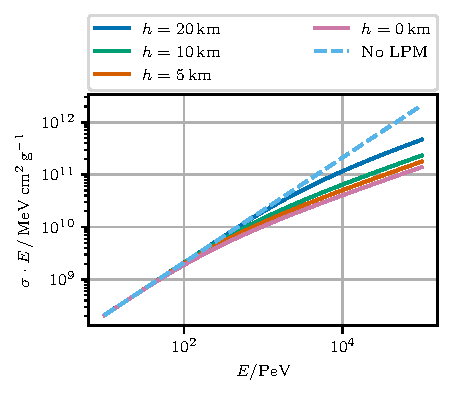
\includegraphics{plots/lpm_cross_photopair_small.pdf}
  \captionof{figure}{Total cross section for electron-positron pair production in air, with the effect of the LPM suppression at different atmospheric heights.}
  \label{fig:lpm_photopair_cross}
\end{minipage}
\end{figure}

\bibliographystyle{JHEP}
\bibliography{references}


%% Full authors list (ONLY FOR COLLABORATIONS)
%\clearpage
%\section*{Full Authors List: \Coll\ Collaboration}
%
%\noindent \textbf{Note comment afterwards:} Collaborations have the possibility to provide an authors list in xml format which will be used while generating the DOI entries making the full authors list searchable in databases like Inspire HEP. \\
%
%\scriptsize
%\noindent
%first.author$^1$, 
%second.author$^2$, 
%third.author$^3$ % .... more names
%and 
%last.author$^{n}$ \\
%
%\noindent
%$^1$first.affiliation.
%$^2$second.affiliation. % .... more affiliation
%$^{m}$last.affiliation.

\end{document}
